\section{Barbalat引理及其推论}\label{3Eref}
类似 \ref{2Dref} 节开头的动机,我们欲在针对非自治系统构造的Lyapunov函数导数仅为负半定时,仍可判断系统的渐近稳定性。
遗憾的是,适用于自治系统的LaSalle不变集原理并不适用于非自治系统。

下面要介绍的Barbalat引理(\ref{barbalat})给出了本身或导数渐近收敛的函数的刻画。
先看一个“否定直觉”的例子。
\begin{example}
    给定对$t$可微的函数$f$,$t \rightarrow \infty$时,$f\to c$  $\nLeftrightarrow $ $\dot{f} \rightarrow 0$!
  \begin{itemize}[leftmargin=1em]
    \item $\nRightarrow $: $f = \mathrm{e}^{- t} \sin (\mathrm{e}^{2 t}) \rightarrow 0$,但是$ \dot{f} = - \mathrm{e}^{- t} \sin
    (\mathrm{e}^{2 t}) + \mathrm{e}^t \cos (\mathrm{e}^{2 t}) \cdot 2 \mathrm{e}^{2 t}$ 无界;    
    \item $\nLeftarrow $:$f = \ln  t$,有$ \dot{f} = \frac{1}{t} \rightarrow0$,但是$f \rightarrow \infty(t \rightarrow \infty)$。
  \end{itemize}
\end{example}
这个例子启示我们,从收敛性不可直接推断导数趋于$0$,需要附加条件。
\begin{definition}[一致连续(uniform continuity)]
    称函数$f(t) : [0,\infty) \rightarrow \mathbb{R}$ 是{\bf 一致连续的(uniformly continuous)}\index{一致连续的(uniformly continuous)},若
     \[\forall \varepsilon > 0, \exists \delta
  = \delta (\varepsilon) > 0, \forall | t_2 - t_1 | \leq \delta \Rightarrow |
  f (t_2) - f (t_1) | \leq \varepsilon\]
\end{definition}
% \begin{lemma}
%     有界闭集(紧集)上的连续函数必是一致连续的。
% \end{lemma}
\begin{theorem}[Barbalat引理]\label{barbalat}\index{Barbalat引理}
    若可微函数$f(t)$当$t\to\infty$时具有有限极限,且$\dot{f}(t)$是一致连续的,那么$\lim\limits_{t\to\infty}\dot{f}(t)=0$。
\end{theorem}

\begin{proof}
  用反证法。假设$\dot{f}(t)$当$t\to\infty$时不收敛至$0$。那么存在$\varepsilon_0>0$使得对$\forall T>0$,均存在无限多个时刻$t_i>T$使得$|\dot{f}(t_i)|\ge \varepsilon_0$。

  因为$\dot{f}(t)$是一致连续的,因此存在$\eta(\varepsilon_0)>0$使得
  \[|\dot{f}(t')-\dot{f}(t'')|<\frac{\varepsilon_0}{2},\forall |t'-t''|<\eta\]
  对于任意$|t-t_i|<\eta$,我们有
  \begin{align*}
    |\dot{f}(t)|&= |\dot{f}(t_i)+\dot{f}(t)-\dot{f}(t_i)|
    \ge |\dot{f}(t_i)|- |\dot{f}(t)-\dot{f}(t_i)|
    >\varepsilon_0-\frac{\varepsilon_0}{2}=\frac{\varepsilon_0}{2}
  \end{align*}
  对于所有$t_i$,均有
  \[\left|\int_{t_i-\eta}^{t_i+\eta}\dot{f}(t)\diff t\right|=\int_{t_i-\eta}^{t_i+\eta}|\dot{f}(t)|\diff t=|f(t_i+\eta)-f(t_i-\eta)|\geq2\eta\cdot\frac{\varepsilon_{0}}{2}=\varepsilon_{0}\eta\]
  第一个等号成立是因为在积分区间内,$\dot{f}(t)$保号。
  
  而$f(t)$具有有限极限,这就意味着存在时刻$T(\varepsilon_0)>0$,使得对于任意$t_2>t_1>T(\varepsilon_0)$,有
 \[|f(t_2)-f(t_1)|<\varepsilon_0\eta\]
  前式与之相矛盾。
\end{proof}
\begin{note}
  第一个条件最常见的两种情况:单调非减(递增)有上界、单调非增(递减)有下界。可微函数一致连续的一个充分条件是其导数有界,因此常通过构造二阶导函数有界的函数以符合第二个条件。

  上述定理的另一种常见表述:
  若$f(t)$是一致连续的,且$\lim\limits_{t\to\infty}\int_{0}^tf(\tau)\diff\tau$存在且有限,那么$\lim\limits_{t\to\infty}{f}(t)=0$。其中,“一致连续”这一条件非常重要。例如,下列并非一致连续的函数$f(t)$的积分随$t\to\infty$存在且有限
  \[\lim_{t\to\infty}\int_0^tf(\tau)\diff \tau=\frac{1}{2}\sum_{n=1}^\infty\frac{1}{n^2}=\frac{\pi^2}{12}\]
  但是$\lim\limits_{t\to\infty}f(t)$并不存在。

  \begin{center}
      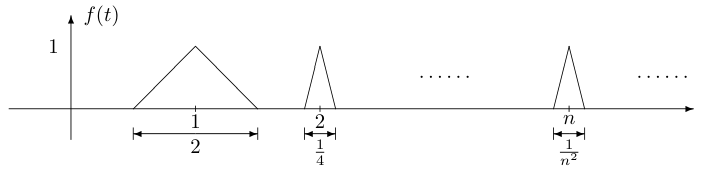
\includegraphics[scale=0.8]{figure/nonlinear/not_uniform_continuous.png}
      \captionsetup{hypcap=false}
      \captionof{figure}{积分具有有限极限,但原函数极限不存在}
  \end{center}
\end{note}
\begin{theorem}[类Lyapunov定理(Lyapunov-like theorem)]\label{Lyapunov-like}\index{类Lyapunov定理(Lyapunov-like theorem)}
  若标量函数 $V(t, x)$ 有下界,且 $\dot{V}(t, x)$ 负半定并一致连续,那么 $\lim\limits_{t \to \infty} \dot{V}(t, x) = 0$。
\end{theorem}
\begin{proof}
  由 $\dot{V}(t, x)$ 负半定,可得 $V (t, x)$ 单调递减,又因为 $V(t, x)$ 有下界,可得 $V (t, x)$ 具有有限极限。此外,$\dot{V}(t, x)$ 一致连续,根据 Barbalat 引理可得 $\lim\limits_{t \to \infty} \dot{V}(t, x) = 0$。
\end{proof}
\begin{example}
  考虑以下非自治系统。在自适应控制中,我们设计控制输入后可能得出形式类似的系统。
  \begin{align*}
    \dot{e} & = - e + \tilde{\theta} \varphi (t)\\
    \dot{\tilde{\theta}} & = - e \varphi (t)
  \end{align*}
  其中 $\varphi (t)$ 是已知的连续有界函数,$e$ 和 $\tilde{\theta}$ 是闭环系统的两个状态,分别代表跟踪误差和参数估计误差。
  
  考虑二次型标量函数 \[V = \frac{1}{2} e^2 + \frac{1}{2} \tilde{\theta}^2\]
  
  显然$V$ 有下界。求$V$的导数
  \begin{align*}
    \dot{V} &= - e^2+e\varphi(t)\tilde{\theta}-\tilde{\theta}\varphi(t)e= - e^2 \leq 0 \\
    \ddot{V} &= - 2 e  \dot{e} = - 2 e (- e + \tilde{\theta} \varphi (t))
  \end{align*}
  
  注意到$\dot{V} \leq 0$ 蕴涵 $V (t) \leq V (0)$,因此 $e, \tilde{\theta}$ 都有界;结合  
   $\varphi (t)$ 有界,可得上述 $\ddot{V}$ 也有界。
  
  因此由 \ref{barbalat} 或 \ref{Lyapunov-like},我们可得 $\lim\limits_{t \rightarrow\infty} \dot{V} (t) = 0$,也就说明了 $\lim\limits_{t \rightarrow \infty} e (t) = 0$。
\end{example}
\begin{theorem}[LaSalle-Yoshizawa定理]\index{LaSalle-Yoshizawa定理}\label{LaSalle-Yoshizawa}
    令$x=0$是 \eqref{freeofnonauto} 的平衡点,并设$f$对$t$是分段连续,且对$x$是局部Lipschitz的(对于$t$是一致的)。令$V$是连续可微函数,满足$\forall t\ge 0,x\in\R{}^n$,\[\gamma_1(\|x\|)\le V(x,t)\le \gamma_2(\|x\|)\]
    \[\begin{aligned}\dot{V}=\frac{\partial V}{\partial t}+\frac{\partial V}{\partial x}f(x,t)\leq-W(x)\leq0\end{aligned}\]
    其中$\gamma_1$和$\gamma_2$是$\mathcal{K}_\infty$类函数且$W$为连续函数。那么  \eqref{freeofnonauto} 的所有解均满足$\lim\limits_{t\to\infty}W(x(t))=0$。
    
    进一步地,若$W(x)$是正定的,那么$x=0$是全局一致渐近稳定的。
\end{theorem}
\begin{note}
  思路导引:(第二行即Barbalat引理的另一种表达形式)
  \[\begin{matrix}
    \text{Barbalat引理}&f\ \text{具有有限极限} & \dot{f}\ \text{一致连续} & \implies & \dot{f}\to 0\\
    &\Updownarrow & \Updownarrow & &\\
    \text{待证结论}&\int^t_0  W (x (\tau)) \diff \tau\ \text{具有有限极限} & W\ \text{对}\ t\ \text{一致连续} & \implies & W(x(t))\to 0\\
    &\Uparrow &\Uparrow && \\
    & \int^t_0  W (x (\tau)) \diff \tau\ \text{单调递增有上界}& W\ \text{对}\ x\ \text{一致连续}&&\\
    &&x\ \text{对}\ t\ \text{一致连续} &&
  \end{matrix}\]
\end{note}
\begin{proof}
  注意到 $W (x) \geq 0$ $\Rightarrow$ $\int^t_0   W (x (\tau)) \diff \tau $单调递增。
  
  由于 $\dot{V} \leq - W (x)$,两边积分得到$V (t) - V (0) \leq - \int^t_0 W (x(\tau)) \diff \tau$,
  进而可知 $\int^t_0 W (x (\tau)) \diff \tau \leq V (0)- V (t) \leq V (0) $。
  因此$\int^t_0 W (x (\tau)) \diff \tau$
  有上界。
  
  于是 $\int^t_0 W (x (\tau)) \diff \tau$ 具有有限极限。
  
  下面证明$W$对$t$一致连续。首先,有界闭集上的连续函数必为一致连续。因此, $W (x)$ 对 $x$一致连续。

  然后,由于 $\dot{V} \leq 0$($V$有上界),且$ \gamma_1 (\| x \|) \leq V (x, t) $($V$有下界),因此
  $V$有界,进而由于$ \gamma_1 (\| x \|) \leq V (x, t) \leq \gamma_2 (\| x \|) $,所以 $\|x\|$也有界,不妨设$\| x \| \leq r$。
  
  由于 $f$ 是局部Lipschitz的,所以对于$\forall t_2 > t_1 \geq 0$,有
  \begin{align*}
    \| x (t_2) - x (t_1) \| & =  \left\| \int^{t_2}_{t_1} f (x (\tau), \tau) \diff
    \tau \right\|\\
    & \leq  L \left| \int^{t_2}_{t_1} \| x (\tau) \| \diff \tau \right|\\
    & \leq  L  r | t_2 - t_1 |
  \end{align*}
  其中$r$为$\|x\|$的最大值(范数是连续函数,紧集上的范数必取得最值)。
  
  对任意使得$\|x(t_2)-x(t_1)\|\le\varepsilon$的$\varepsilon>0$,取$|t_2-t_1|\le\frac{\varepsilon}{Lr}\triangleq\delta>0$即可。
  因此 $x (t)$ 对 $t$是一致连续的,进而$W (x)$对 $t$是一致连续的。
  
  综上,由Barbalat引理可知 $\lim\limits_{t \rightarrow \infty} W (x (t)) =  0$。
\end{proof}
\newpage
\begin{definition}
设$x(t)$是关于时间的函数。
\begin{itemize}[leftmargin=1em]
    \item $L_p$($p\in[1,\infty)$)范数$\|x\|_p$定义为
  \begin{align*}
  \|x\|_p=\left(\int_0^{\infty}|x(\tau)|^p\mbox{d}\tau\right)^{\frac{1}{p}},
  \end{align*}
  \item 无穷范数$\|x\|_{\infty}$定义为
   \begin{align*}
  \|x\|_{\infty}=\sup_{t\geq 0} |x(t)|.
  \end{align*}
  \item 若$\|x\|_p$存在(有界),则称 $x\in\mathbb{L}_p$。
\end{itemize}
 注:在本定义中,使用$|x|$来表示$x$的绝对值(若$x$为标量)或$x$的欧几里得范数(若$x$为向量)。
\end{definition}
\begin{corollary}\label{barbalat_cor_1}
  若连续可微函数$x(t)\in \mathbb{L}_p\cap \mathbb{L}_\infty$($p\in[1,\infty)$),且$\dot{x}\in \mathbb{L}_\infty$,则$\lim\limits_{t \rightarrow \infty}x(t)=0$。
\end{corollary}
证明略。
\begin{note}
  思路导引:
  \[\begin{matrix}
    \text{Barbalat引理}&f\ \text{具有有限极限} & \dot{f}\ \text{一致连续} & \implies & \dot{f}\to 0\\
    &\Updownarrow & \Updownarrow & &\\
    \text{待证结论}&\int^t_0  x^p (\tau) \diff \tau\ \text{具有有限极限} & x^p\ \text{对}\ t\ \text{一致连续} & \implies & x^p\to 0 \implies x\to 0\\
    &\Uparrow &\Uparrow && \\
    & x\in\mathbb{L}_p\ \text{的定义}& \frac{\diff x^p}{\diff t}\ \text{有界}&\Leftarrow&x,\dot{x}\in \mathbb{L}_\infty
  \end{matrix}\]
\end{note}
% \begin{corollary}\label{barbalat_cor_2}
%   若连续可微函数$x(t)\in \mathbb{L}_1\cap \mathbb{L}_\infty$,且$\dot{x}\in \mathbb{L}_\infty$,则$\lim\limits_{t \rightarrow \infty}x(t)=0$。
% \end{corollary}
% \begin{hint}
%     \[\int^t_0  x^2 (\tau)\diff \tau\le \max(|x(t)|)\int^t_0  |x (\tau)|\diff \tau<\infty\]
%     能提出第一项是由于$x(t)$有界。之后遵循证明上个推论的思路即可。
% \end{hint}